%!xelatex = 'xelatex --halt-on-error %O %S'

\documentclass{buaaemp}
\begin{document}

% 标题,作者
\emptitle{变温霍尔效应}
\empauthor{智朝晖}{李文萍}

% 奇数页页眉 % 请在这里写出第一作者以及论文题目
\fancyhead[CO]{{\footnotesize 智朝晖: 变温霍尔效应}}


%%%%%%%%%%%%%%%%%%%%%%%%%%%%%%%%%%%%%%%%%%%%%%%%%%%%%%%%%%%%%%%%
% 关键词 摘要 首页脚注
%%%%%%%%关键词
\Keyword{\quad 霍尔效应\quad 霍尔系数\quad 电阻率\quad 范德堡法}
\twocolumn[
\begin{@twocolumnfalse}
\maketitle

%%%%%%%%摘要
\begin{empAbstract}
本实验使用NDWH-648型变温霍尔效应实验仪(温度范围77.3K-300K)利用范德堡法测量了高阻样品InSb在$-196\textcelsius\sim$室温下的霍尔系数及电阻率,并且通过磁场换向、电流换向消除了诸多热磁副效应。根据霍尔系数的符号确定了载流子的类型,并且确定了载流子浓度$p$和$n$及迁移率$\mu$等基本参量。

\end{empAbstract}

%%%%%%%%首页角注,依次为实验时间、报告时间、学号、email
\empfirstfoot{2022-10-06}{2022-10-06}{20377365}{20377365@buaa.edu.cn}
\end{@twocolumnfalse}
]
%%%%%%%%!首页角注可能与正文重叠,请通过调整正文中第一页的\enlargethispage{-3.3cm}位置手动校准正文底部位置:
%%%%%%%%%%%%%%%%%%%%%%%%%%%%%%%%%%%%%%%%%%%%%%%%%%%%%%%%%%%%%%%%
%  正文由此开始
\wuhao 
%  分栏开始

\section{引~~言}
半导体是一种电导率介于导体和绝缘体之间的物质。半导体在现代社会中具有重要应用,诸如计算机之类的电子产品的核心单元都是利用半导体的电导率变化来处理信息。其中,硅作为第一代半导体材料,发挥了不可替代的作用。因此,测量硅的电导率等特性具有重要意义。
	
早在19世纪,人们就观察到了半导体的许多非同寻常的性质。例如,法拉第(Michael Faraday)于1833年发现,随着温度的升高,AgS的电导率会增加\cite{laeri2006host},而金属的电导率则会下降。
	
	
虽然电导率的实验测量已经成为研究半导体的基本方法,但是由于影响电导率的因素有很多,仅仅依靠电导率不足以做更深入的分析。霍尔效应最初是1879年由霍尔(E.H. Hall)在金属中发现的,但是在半导体中这个效应更为显著,而且能为深入分析半导体提供重要依据\cite{solidstatephysics}。
	
霍尔效应在当时并未得到解释,直到1897年约瑟夫·汤姆逊(Joseph John Thomson)发现电子,人们便自然猜想,霍尔效应的出现是由于电子在磁场下偏转并积累到样品两端,形成霍尔电压。



虽然这一经典理论可以解释从实验得到的关于碱金属与某些其它金属的霍尔系数,它不能解释载流子的正负电性。真正使得霍尔效应得到圆满解释的是20世纪发展起来的固体理论。\pagebreak 1929年,鲁道夫·佩尔斯(Rudolf Ernst Peierls)对于正霍尔效应给出理论解释。在正霍尔效应里,电流载子带有正价。佩尔斯表示,这是因为在能带边缘区域的电子,其物理行为貌似带有正价\cite{peierls1929theorie}。1931年,威尔逊(Alan Herries Wilson)总结了前人的工作,对晶体为什么会出现金属、半导体、绝缘体之分做了详细解释,并且强调了杂质对于半导体导电性质的影响\cite{wilson1931theory}。利用霍尔效应可以确定半导体的导电类型和载流子浓度,利用霍尔系数和电导率的联合测量,可以用来研究半导体的导电机理(本征导电和杂质导电)和散射机理(晶格散射和杂质散射),进一步确定半导体的迁移率、禁带宽度、杂质电离能等基本参数。测量霍尔系数随温度的变化,可以确定半导体的禁带宽度、杂质电离能即迁移率的温度特性。
	
然而,如何精确地测量给定样品的电阻率和霍尔系数,是一个技术上的难题。在1958年,范德堡(Van der Pauw)提出了范德堡测量法(又称四点量测法),它能够用于精确测量任意形状的样品,只需要样品很薄、无孔、边上可以连接电极\cite{philips1958method}。
	
本实验将利用这一方法,测量从$-196\textcelsius\sim$室温温度范围内InSb半导体薄片样品的电阻率和霍尔系数,并确定载流子的种类、浓度以及随温度变化的关系;利用测量的数据,还将分析出载流子的迁移率、净杂质浓度等材料的基本参数。

\section{原~~理}
\subsection{霍尔效应}

	如图\ref{halleffect}所示,霍尔效应指的是将一个通有电流的金属导体放置于垂直于电流方向的磁场中时,在导体的平行于电流和磁场的两个侧面之间可以测量到电势差,其正负取决于载流子的种类。霍尔效应出现的原因可以简要理解为:在磁场的作用下,导体中的载流子发生偏转,聚集到导体的侧面,从而产生霍尔电势差。
	\begin{figure}[!htbp]
		\centering
		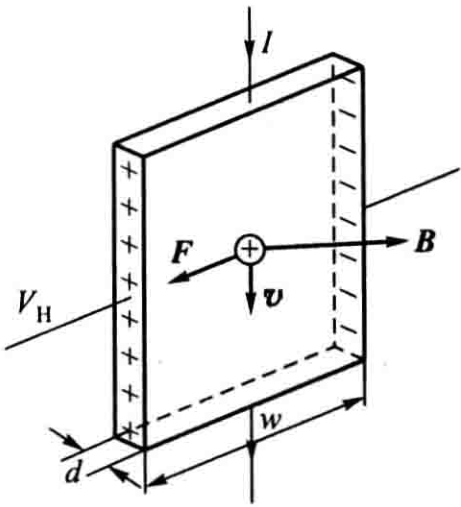
\includegraphics[width=0.3\linewidth]{./image/halleffect.png}
		\caption{霍尔效应示意图}
		\label{halleffect}
	\end{figure}

	霍尔系数$R_H$的定义为:$V_H=R_H\frac{IB}{d}$,$d$为样品厚度,$B$为磁感应强度,$I$为电流,$V_H$为霍尔电压。
	根据基本的Drude Model平衡时电场力和洛伦兹力抵消可知,在p型半导体中,$V_H=\frac{IB}{pqd}$,$p$为空穴浓度,$q$为载流子带电量。于是霍尔系数可以表示为:$R_H=\frac{1}{pq}=\frac{V_H d}{IB}$。而在含有两种载流子的样品中,可以证明\cite{solidstatephysics}:
	\begin{equation}
		R_{\mathrm{H}}=\frac{3 \pi\left(p \mu_{\mathrm{p}}^{2}-n \mu_{\mathrm{n}}^{2}\right)}{8 q\left(p \mu_{\mathrm{p}}+n \mu_{\mathrm{n}}\right)^{2}}
		\label{equation:hall}
	\end{equation}
	
	其中$n$为电子浓度,$\mu_p$和$\mu_n$分别为空穴和电子的迁移率。
 
	\subsection{范德堡法测量电阻率和霍尔系数}
	本实验利用范德堡法测量给定样品的电阻率和霍尔系数。如图\ref{fourpoint}所示,1、2、3、4代表四个接触点,则电阻率可以表示为\cite{钱建强2016近代物理实验}:
	\begin{figure}[htbp]
		\centering
		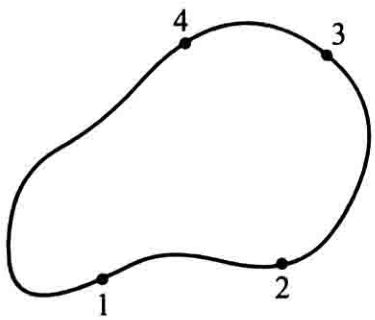
\includegraphics[width=0.3\linewidth]{./image/fourpoint.png}
		\caption{利用范德堡法测量电阻率}
		\label{fourpoint}
	\end{figure}
 
	\begin{equation}
		\centering
		\rho=\frac{\pi d}{ln2}\frac{R_{12,34}+R_{23,41}}{2}f
	\end{equation}

	其中
	\begin{equation}
		\centering
		R_{12,34}=\frac{V_{4}-V_{3}}{i_{12}}, \quad R_{23,41}=\frac{V_{1}-V_{4}}{i_{23}}
	\end{equation}

	以及
	\begin{equation}
		\cosh \left\{\frac{\left(R_{12,34} / R_{23,41}-1\right)}{\left(R_{12,34} / R_{23,41}+1\right)} \frac{\ln 2}{f}\right\}=\frac{1}{2} \exp \left(\frac{\ln 2}{f}\right)
	\end{equation}

	垂直于样品表面加一磁场,电流自1端流向3端,则霍尔系数为:
	\begin{equation}
		R_{\mathrm{H}}=\frac{d}{B} \Delta R_{13,24}=\frac{d}{B} \frac{\Delta\left(V_{4}-V_{2}\right)}{i_{13}}
	\end{equation}

	式中$\Delta\left(V_{4}-V_{2}\right)$表示加磁场后4端与2端电位差的变化。

 
	\section{实验过程}
	本实验利用NDWH-648型变温霍尔效应实验仪(温度范围77.3K-300K)进行温度控制、提供霍尔电流、测量霍尔电压,并利用$PZ93A$型直流数字电压表测量铜-康铜热电偶热电势,对照实验室提供的表格得出样品的温度。实验装置及样品的一些基本参数见表\ref{apparatus}:
	\begin{table}[htbp]
		\centering
		\begin{tabular}{ccc}%表格中的数据居中,c的个数为表格的列数
			\hline\hline\noalign{\smallskip}
			项目 & 数值 & 单位  \\
			\noalign{\smallskip}\hline\noalign{\smallskip}
			室温 & $24.3$ & $\textcelsius$ \\
			磁场强度 & $0.402$ & $T$ \\
			样品厚度 & $1.00\pm0.02$ & $mm$ \\
			霍尔电流 & $100.00\pm0.01$ & $\mu A$ \\
			霍尔电压计量程 & $2$ & $V$ \\
			\noalign{\smallskip}\hline\hline
		\end{tabular}
		\caption{实验装置及样品的基本参数}
		\label{apparatus}
	\end{table}
	
	由于存在多种热磁副效应,因此实验中通过改变霍尔电流和磁场的方向进行测量并取平均值以消除它们的影响。
	
	按照实验室提供的表格上所列出的设定温度,将样品插入液氮瓶中冷却至77.3K稳定后迅速抽出放至实验平台上,设置励磁电流基本恒定开始记录温度与霍尔电势的关系,当温度稳定至室温后开始搜集电势电压随着磁场的变化关系,同时搜集伏安特性曲线。结果如下。
\section{数据记录}
\subsection{霍尔电势和温度变化关系}
如图所示\ref{fig:temp_magnetic}\ref{fig:repaint}
\begin{figure}
    \centering
    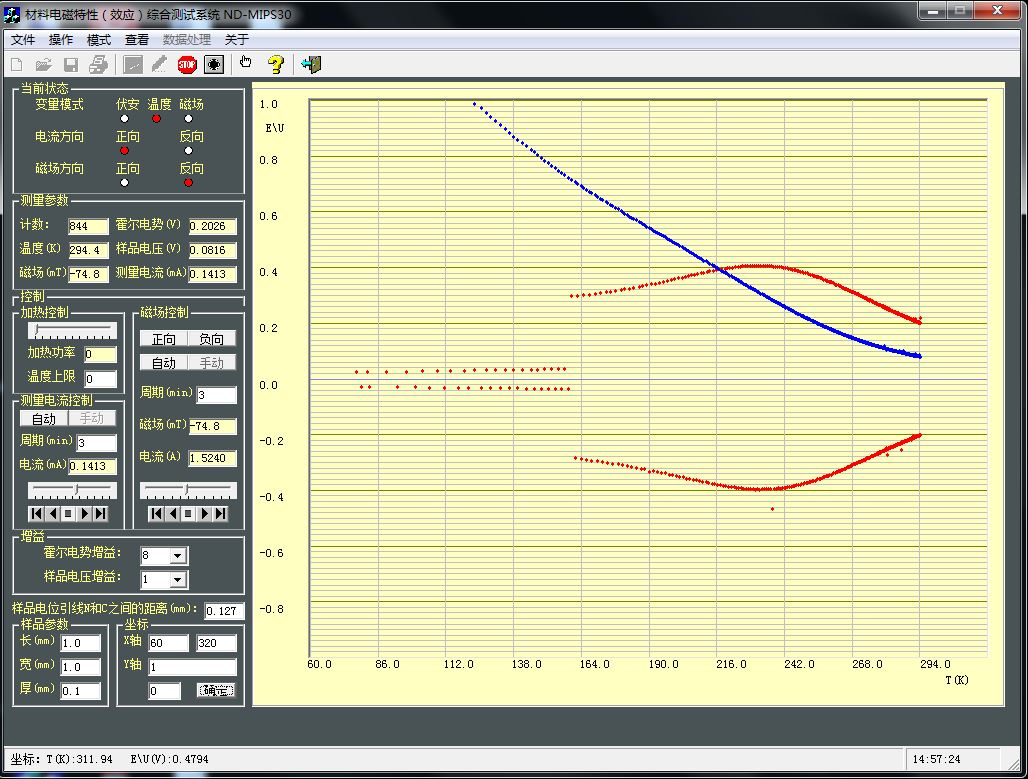
\includegraphics[width=\linewidth]{image/1.jpg}
    \caption{仪器扫描霍尔电势随温度变化关系}
    \label{fig:temp_magnetic}
\end{figure}

\begin{figure}
    \centering
    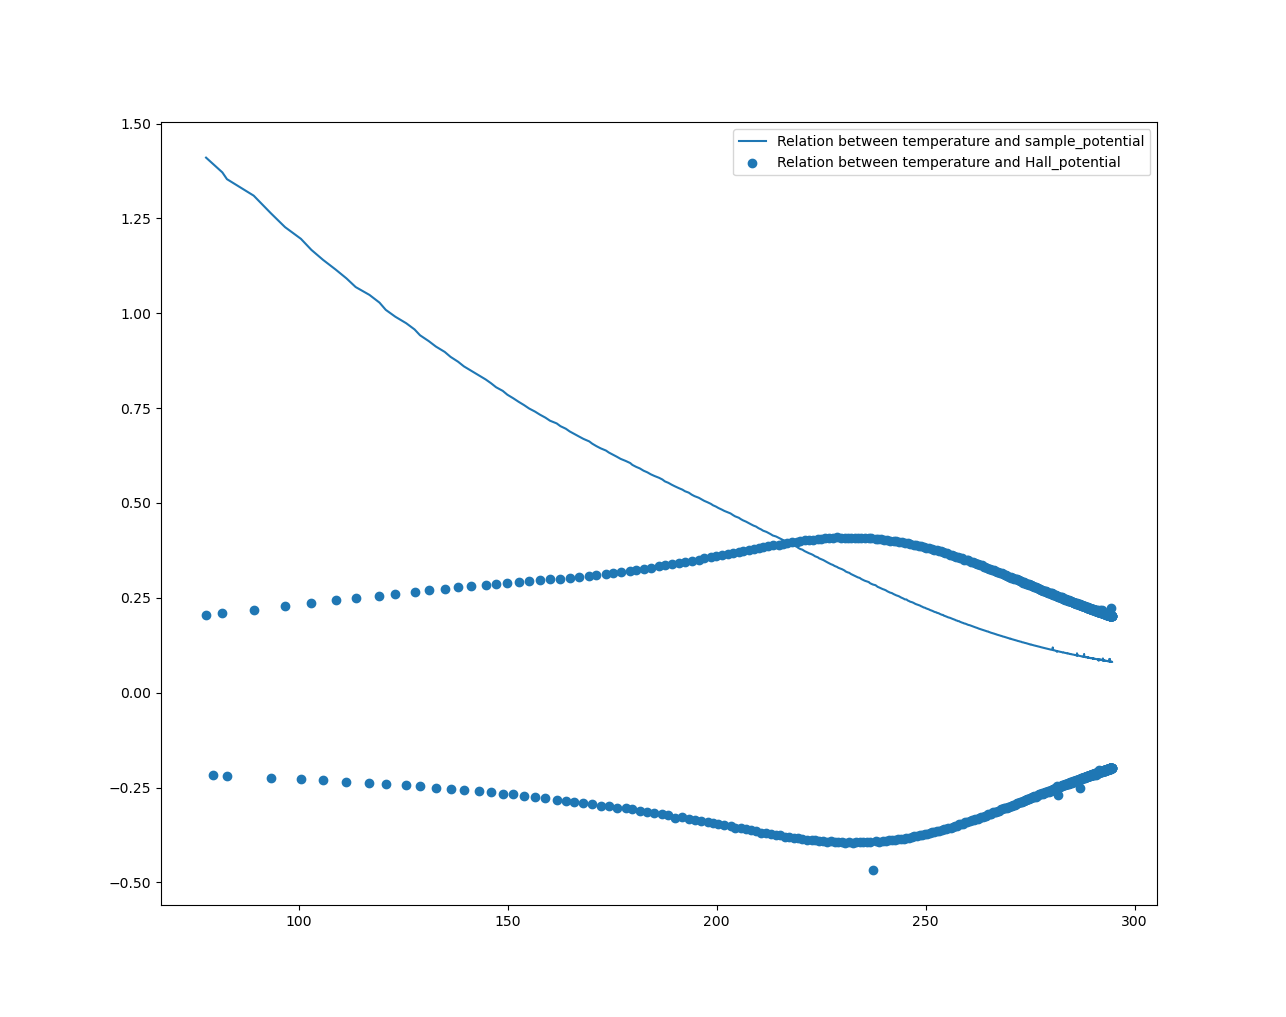
\includegraphics[width=\linewidth]{image/Potential_Temp.png}
    \caption{上述结果记录数据重绘制}
    \label{fig:repaint}
\end{figure}

\subsection{霍尔电势随着磁场变化关系}
如图所示\ref{fig:potential_B}
\begin{figure}
    \centering
    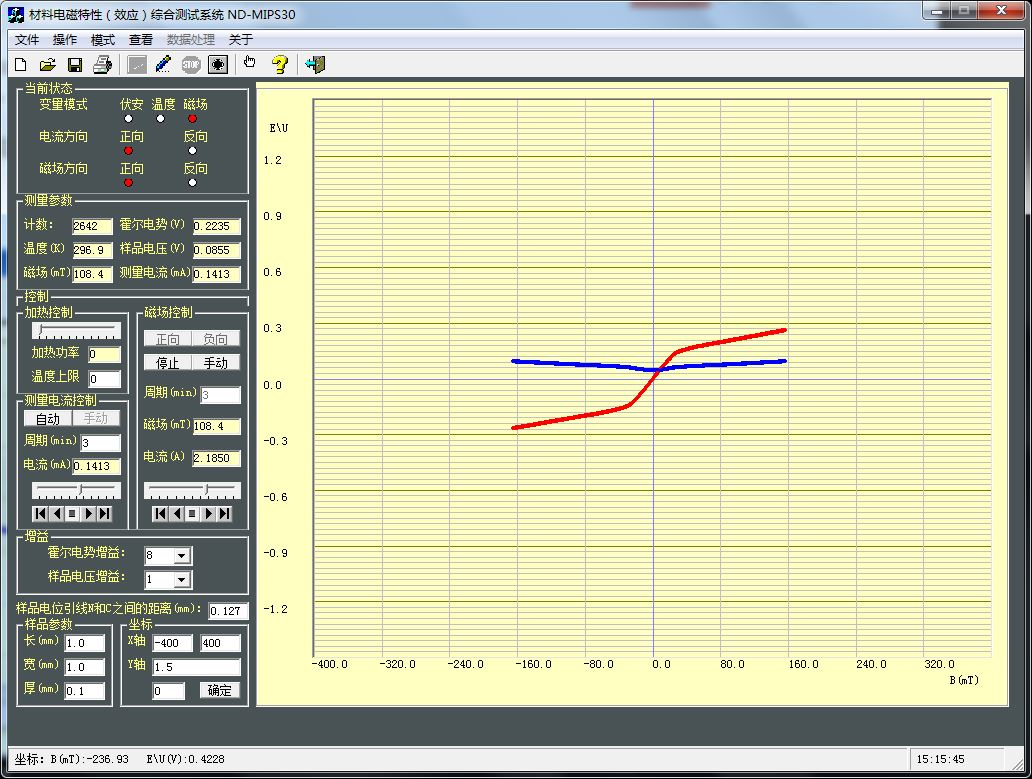
\includegraphics[width=\linewidth]{image/temp.jpg}
    \caption{霍尔电势随着磁场变化关系}
    \label{fig:potential_B}
\end{figure}

\subsection{稳定后的伏安特性曲线}
如图所示\ref{fig:VA}
\begin{figure}
    \centering
    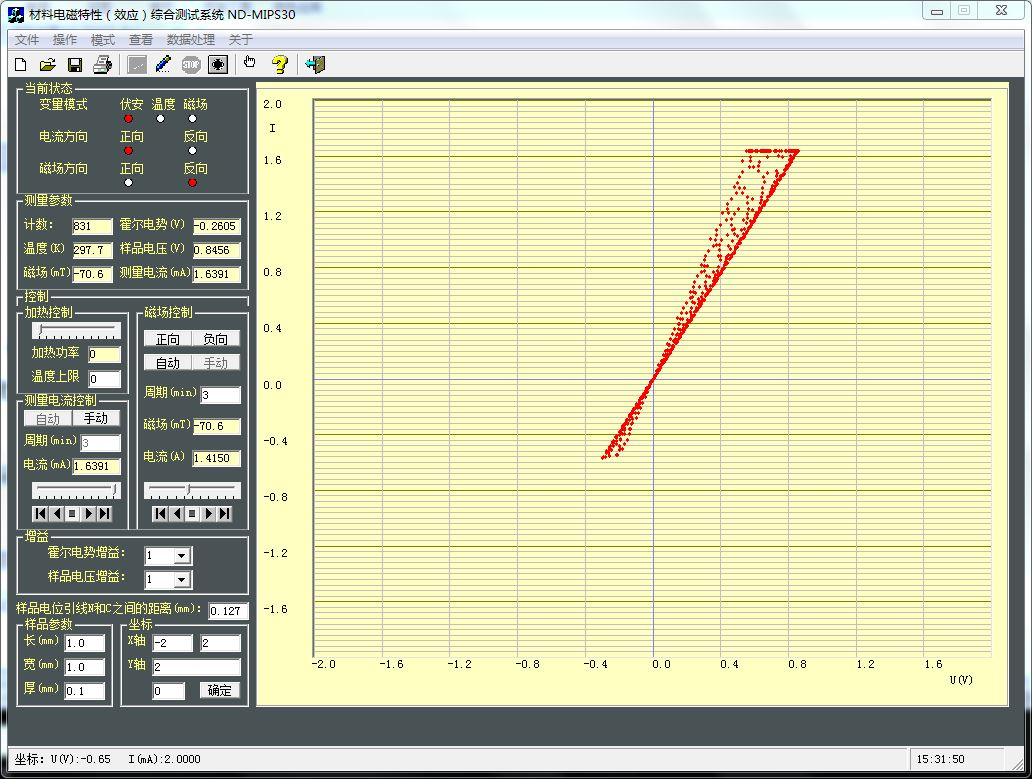
\includegraphics[width=\linewidth]{image/VA.jpg}
    \caption{稳定后的伏安特性曲线}
    \label{fig:VA}
\end{figure}

\section{数据处理及分析}
实验过程中保持磁场方向垂直于样品表面,通过样品的电流恒定为$I=141.20\mu A$,电流的波动不超过$0.1\mu A$。利用公式可以计算得出电阻率,并且绘制出了“电导率-温度倒数”关系图\ref{fig:Conductivity}和“霍尔效应系数-温度倒数”\ref{fig:Hall_coefficient}关系图,与书上的霍尔系数关系图对比。

\begin{figure}
    \centering
    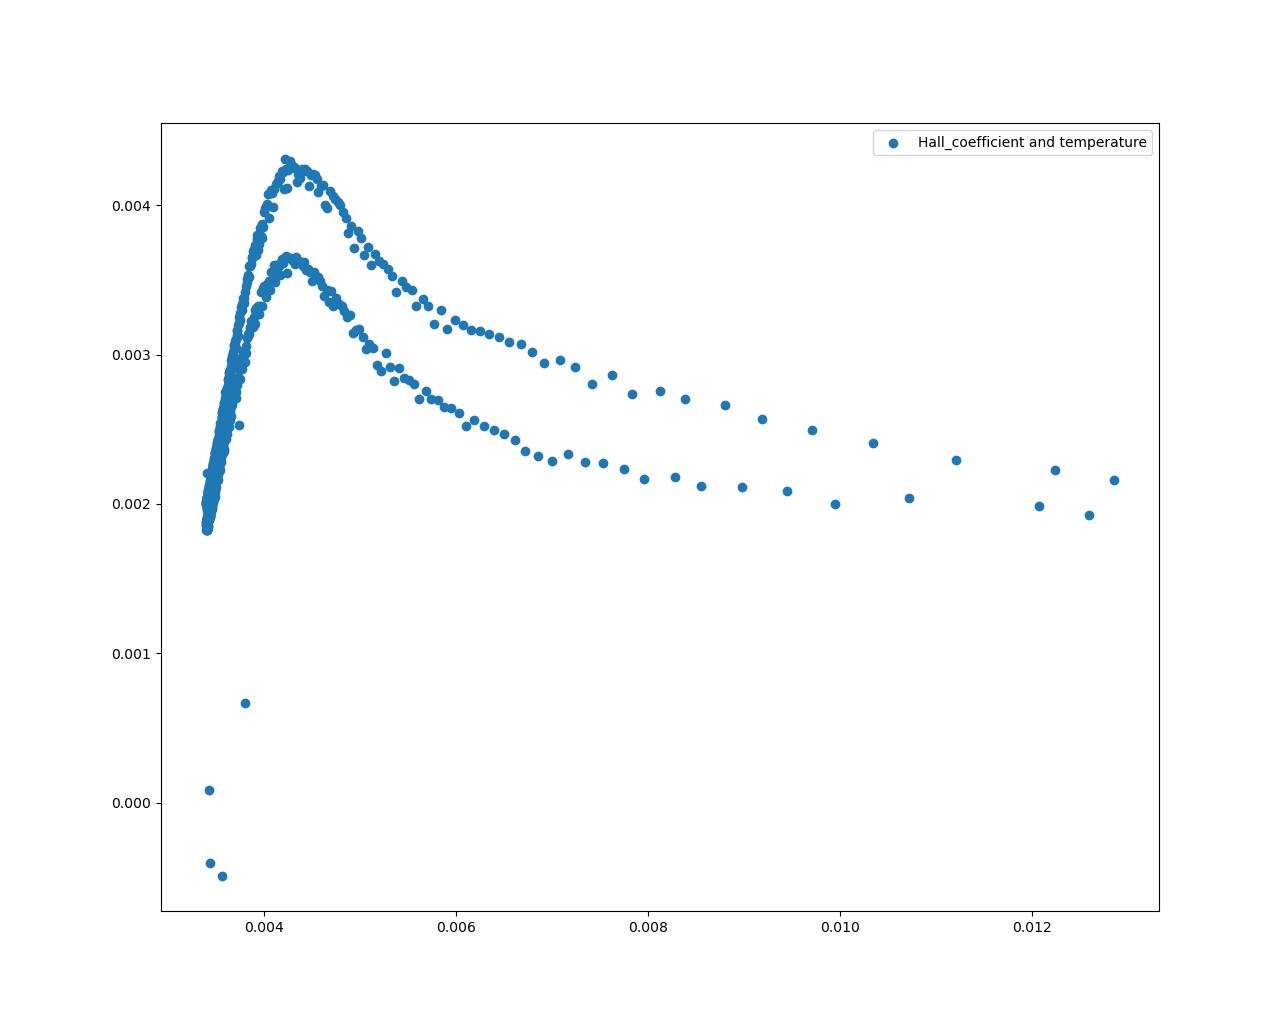
\includegraphics[width=\linewidth]{image/Hall_coefficient.png}
    \caption{霍尔效应系数-温度倒数}
    \label{fig:Hall_coefficient}
\end{figure}

\begin{figure}
    \centering
    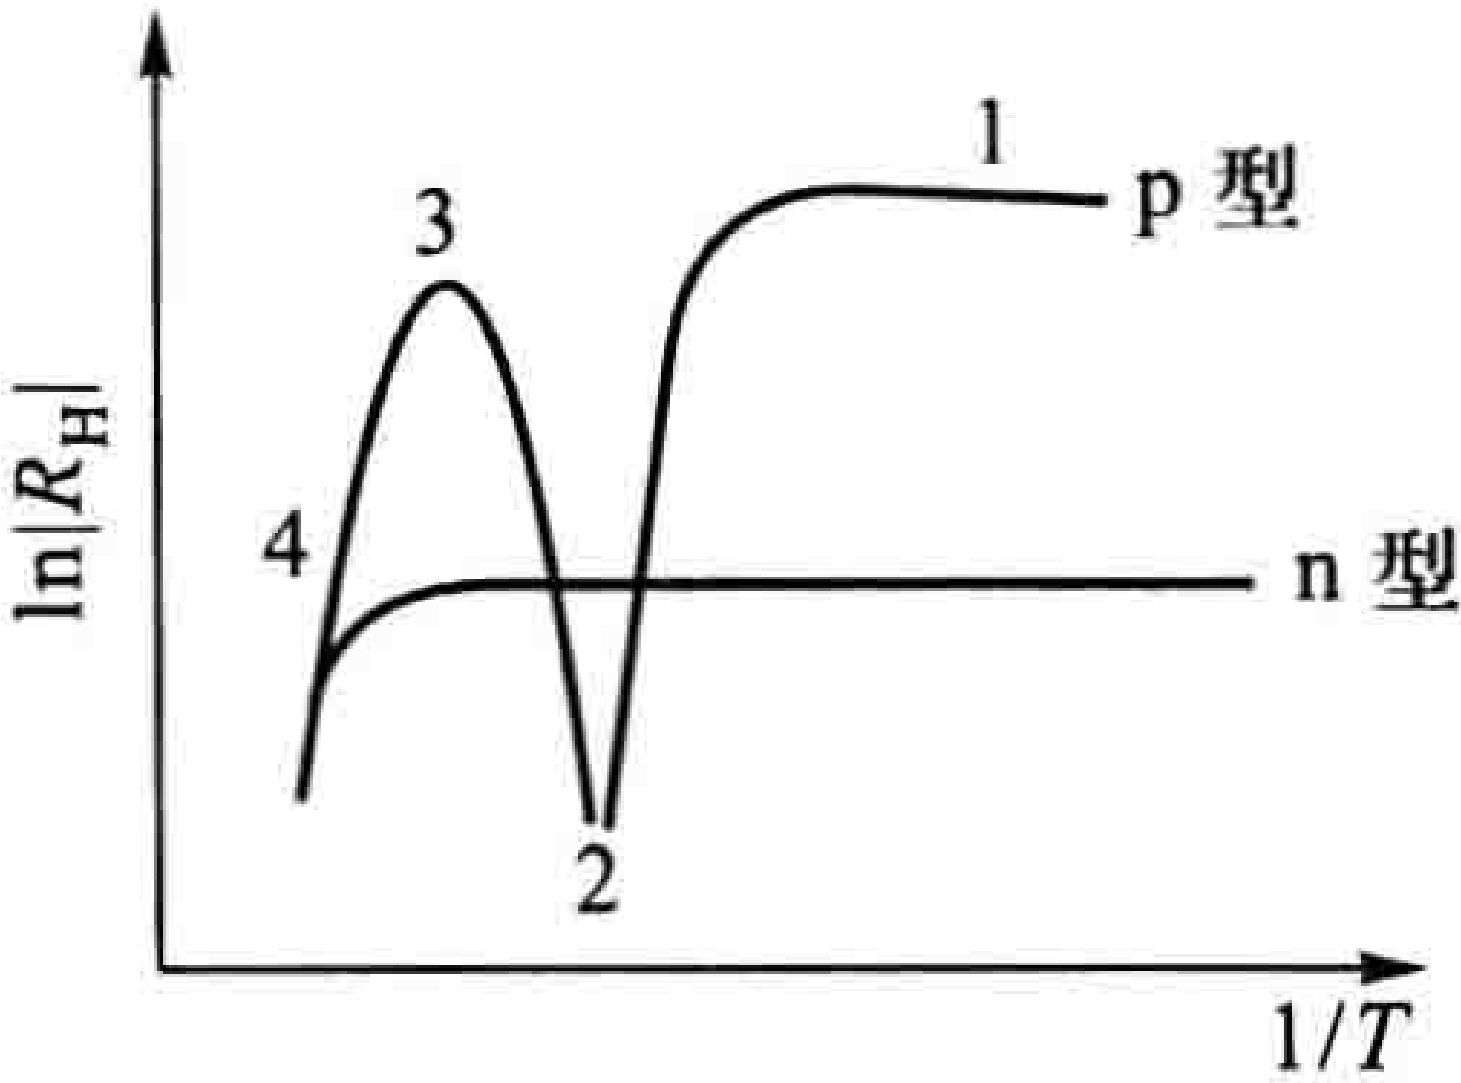
\includegraphics[width=\linewidth]{image/bookhall.png}
    \caption{书上的霍尔系数图}
    \label{fig:bookhall}
\end{figure}

\begin{figure}
    \centering
    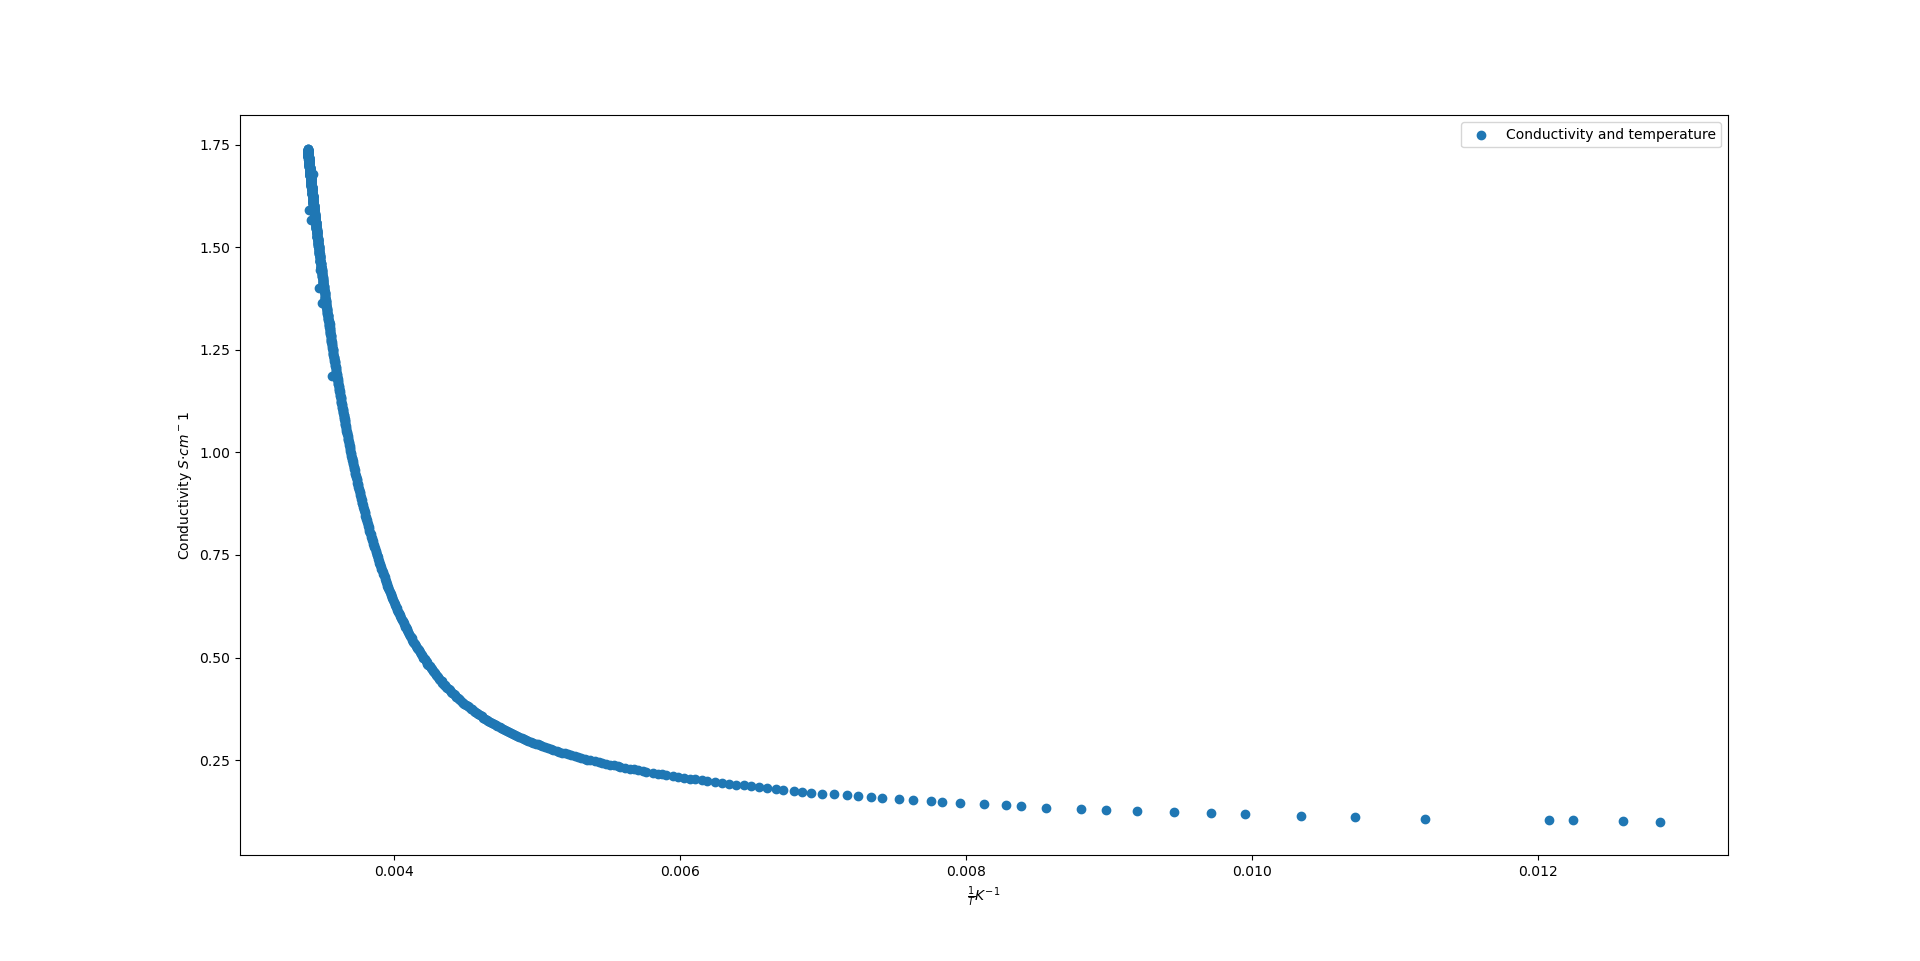
\includegraphics[width=\linewidth]{image/Conductivity.png}
    \caption{电导率-温度倒数}
    \label{fig:Conductivity}
\end{figure}

\begin{figure}
    \centering
    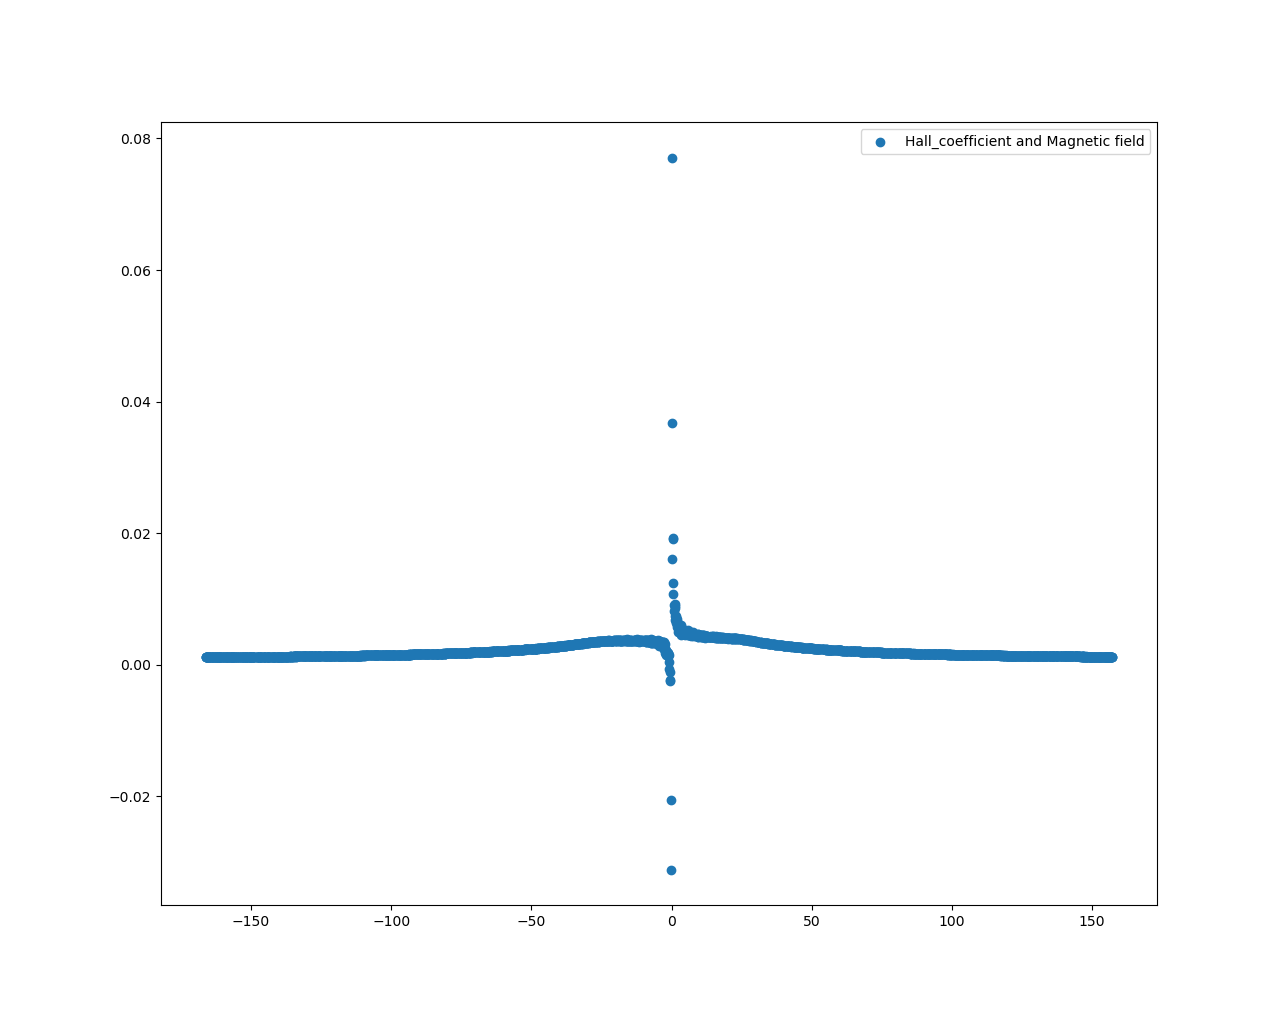
\includegraphics[width=\linewidth]{image/Hall_coefficient_B.png}
    \caption{霍尔系数和磁场的关系}
    \label{fig:Hall_B}
\end{figure}
	理论分析可知,对于图\ref{fig:bookhall},1表示杂质尚未完全电离的区域,随着温度的升高,杂质电离增加,空穴浓度增大,杂质散射减小,迁移率增大,因此电导率增加;2表示杂质电离饱和区,此时本征激发尚不明显,随温度升高,载流子浓度不变,但晶格散射增大导致迁移率下降,因此电导率下降;3表示本征激发的高温区,本征激发产生的载流子随温度指数增加,远大于散射引起的迁移率下降(按照温度的幂次)效应,因此电导率急剧增长。
	
	实际测量时,由于起始温度不够低,因此测量得到的曲线只对应了教材上图像的2、3区域。同时因为升温过快在杂志饱和点附近没有细致采样,导致未出现信号峰。图像中杂质电离饱和区的温度范围为:
	\begin{center}
		$130K\le T\le160K$
	\end{center}
	
	利用教材上给出的公式,可以算得在杂质电离饱和区不同温度下的电子空穴迁移率比值$b$,由记录数据我们可以得知 $R_s=-0.00224 m^3/C$,信号峰 $R_s=0.0042 m^3/C$,得到 $b=0.1065$,本征激发后载流子为空穴。



\section{结~~论}
本实验使用NDWH-648型变温霍尔效应实验仪(温度范围77.3K-300K)利用范德堡法测量了高阻样品InSb在$-196\textcelsius\sim$室温下的霍尔系数及电阻率,并且通过磁场换向、电流换向消除了诸多热磁副效应。根据霍尔系数的符号确定本征激发后为空穴导电,并且确定了电子空穴迁移率比$\mu$等基本参量。同时绘制了霍尔系数-温度特性曲线、电导率-温度特性曲线以及霍尔系数随磁场强度变化曲线。实验结果表明,而在温度升至约$160K$时进入本征激发区。电阻率和霍尔系数随温度的变化与理论相符。

%%%%%%%%%%%%%%%%%%%%%%%%%%%%%%%%%%%%%%%%%%%%%%%%%%%%%%%%%%%%%%%%
%  参考文献
%%%%%%%%%%%%%%%%%%%%%%%%%%%%%%%%%%%%%%%%%%%%%%%%%%%%%%%%%%%%%%%%
%  参考文献按GB/T 7714-2015《文后参考文献著录规则》的要求著录. 
%  参考文献在正文中的引用方法:\cite{bib文件条目的第一行}

\renewcommand\refname{\heiti\wuhao\centerline{参考文献}\global\def\refname{参考文献}}
\vskip 12pt

\let\OLDthebibliography\thebibliography
\renewcommand\thebibliography[1]{
  \OLDthebibliography{#1}
  \setlength{\parskip}{0pt}
  \setlength{\itemsep}{0pt plus 0.3ex}
}

{
\renewcommand{\baselinestretch}{0.9}
\liuhao
\bibliographystyle{gbt7714-numerical}
\bibliography{./TempExample}
}


\end{document}
